\documentclass[../main.tex]{subfiles}
\begin{document}
\section{Results}\label{results}
%oppgave 5b)
\subsection{Euler and Verlet without object orientation}\label{sec:results-euler-verlet}
In order to make sure that our algorithm is running correctly, we started by solving the differential equation using both Euler's and Verlet's method without using object oriented(oo) code. The algorithms used to calculate the two are located in the following folders: \href{https://github.com/kmaasrud/Project-5/tree/master/code/Earth-Sun_Euler-FWD}{\textsc{/code/Earth-Sun\_Euler-FWD}} and \href{https://github.com/kmaasrud/Project-5/tree/master/code/Earth-Sun_Verlet}{\textsc{/code/Earth-Sun\_Verlet}}.

\begin{figure}[!h]
  \centering
  \makebox[\textwidth][c]{
  \begin{minipage}{0.6\textwidth}
        \centering
        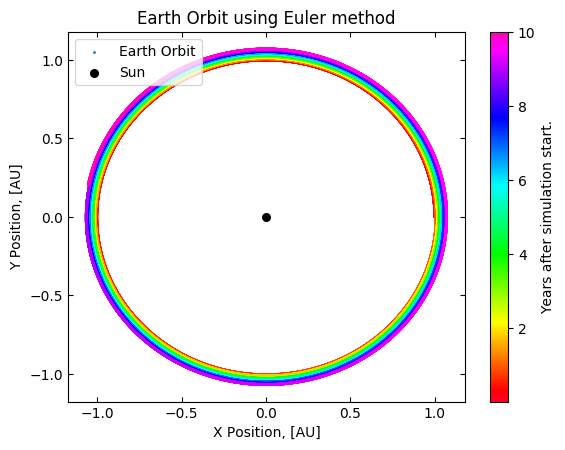
\includegraphics[width=1\textwidth]{EarthOrbit_Euler.png} % first figure itself
    \end{minipage}\hfill
    \begin{minipage}{0.6\textwidth}
        \centering
        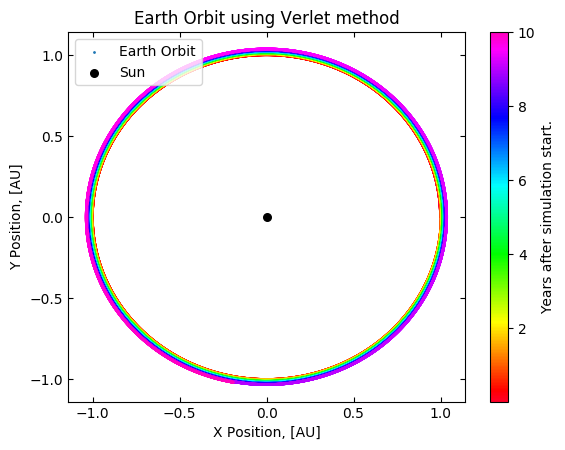
\includegraphics[width=1\textwidth]{EarthOrbit_Verlet.png} % second figure itself
    \end{minipage}
}
  \caption{Earth orbit around the Sun using Eulers method and Verlets method respectively }
  \label{fig:EarthOrbit_Euler_Verlet}
\end{figure}
\FloatBarrier

%oppgave 5c)
\subsection{Testing}
\subsubsection{Stability with varying timestep} \label{sec:results-test-timestep}
In the figures below we plotted Earths orbit over a thousand years with different timesteps.

\begin{figure}[!h]
  \centering
  \makebox[\textwidth][c]{
  \begin{minipage}{0.7\textwidth}
        \centering
        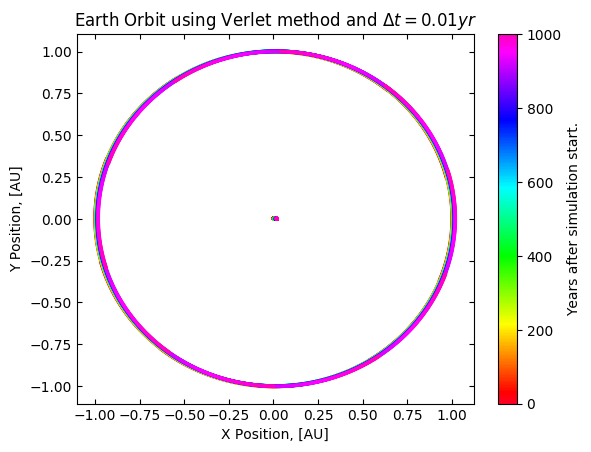
\includegraphics[width=1\textwidth]{/test/Earth-Sun_Test0-01.png} % first figure itself
    \end{minipage}\hfill
    \begin{minipage}{0.7\textwidth}
        \centering
        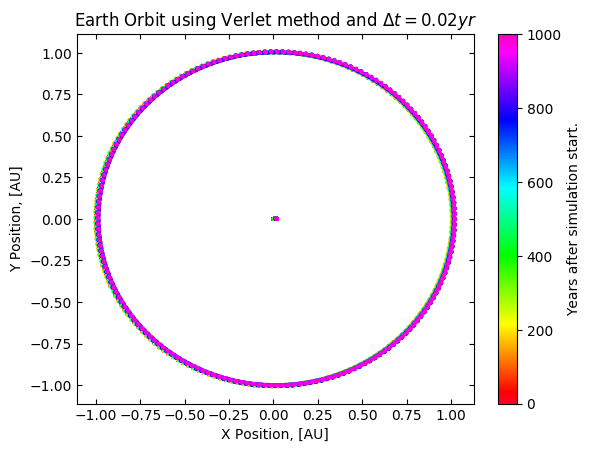
\includegraphics[width=1\textwidth]{/test/Earth-Sun_Test0-02.png} % second figure itself
    \end{minipage}
}
  \caption{Earth orbit with time steps $\Delta t = 0.01$years and $0.02$years respectively }
  \label{fig:results-Timestep1}
\end{figure}
\FloatBarrier
\begin{figure}[!h]
  \centering
  \makebox[\textwidth][c]{
  \begin{minipage}{0.7\textwidth}
        \centering
        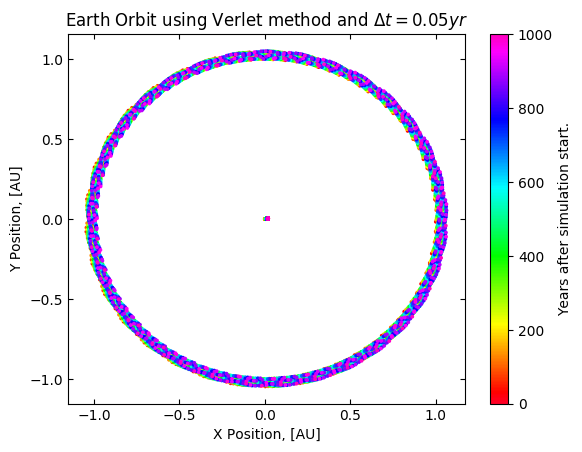
\includegraphics[width=1\textwidth]{/test/Earth-Sun_Test0-05.png} % first figure itself
    \end{minipage}\hfill
    \begin{minipage}{0.7\textwidth}
        \centering
        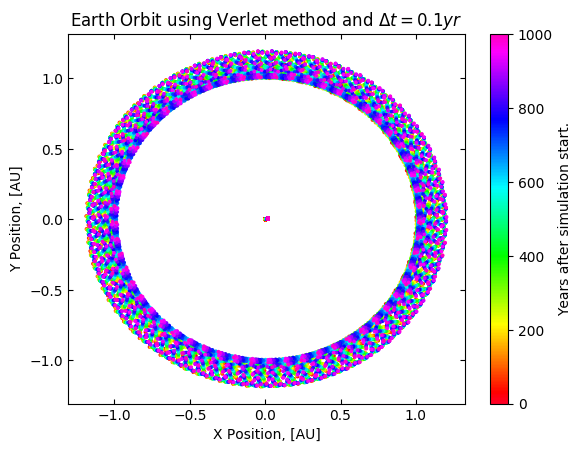
\includegraphics[width=1\textwidth]{/test/Earth-Sun_Test0-1.png} % second figure itself
    \end{minipage}
}
  \caption{Earth orbit with time steps $\Delta t = 0.05$year and $0.1$year respectively }
  \label{fig:results-Timestep2}
\end{figure}
\FloatBarrier

\subsubsection{Energy and angular momentum conservation}\label{sec:results-test-conservation}
In the figures below, kinetic energy and potential energy is plotted as a function of time in the system. We chose to simulate over a thousand years with a timestep of $\Delta t = 0.01$, as this timestep is sufficient.
\begin{figure}[!h]
  \centering
  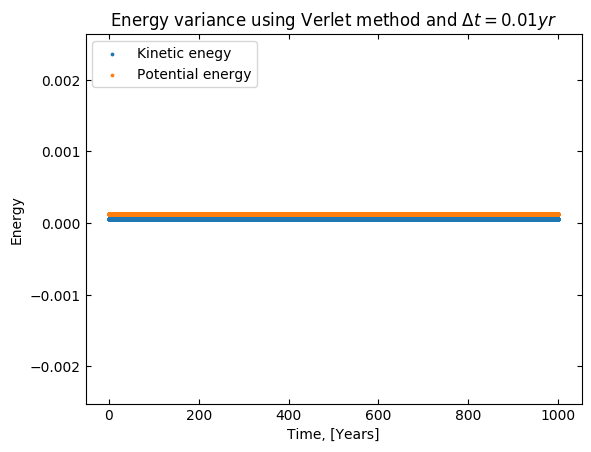
\includegraphics[width=1\textwidth]{/test/Energy_Test.png} % first figure itself
  \caption{Kinetic and Potential energy with timestep $\Delta t = 0.01$year.}
  \label{fig:results-Energies}
\end{figure}
\FloatBarrier

\subsubsection{Verlet vs. Euler}\label{sec:Verlet_VS_Euler}
\begin{table}[!h]
  \caption{Comparison of flops and time for the Verlet and Euler method for $10^6$ iterations over a period of 100 years simulating all planets}
  \centering
  \begin{tabular}{l r r}
                            &\textbf{Flops}&\textbf{Time spent}\\
                            \hline
    \textit{With filesave} & & \\
    Euler's method:          &  10N & 126 s\\
    Verlet's method:          & 6N  & 119 s\\
    \hline
    \textit{Without filesave} & & \\
    Euler's method:          &  10N & 67 s\\
    Verlet's method:          & 6N  & 71 s\\
  \end{tabular}
  \label{tab:EulervsVerlet}
  \end{table}
\FloatBarrier

%oppgave 5 d)
\subsection{Escape velocity} \label{sec:results-esc-vel}
By trail and error we found that the escape velocity of planet Earth is somewhere around $2.828 \pi$, which is pretty close to the theoretical value calculated below.
From section \ref{sec:theory-EscapeVelocity} using equation \eqref{eq:escapevelocity} to calculate the  theoretical value $$v_{esc-theoretical} = \sqrt{\frac{2\cdot4\pi^2\cdot1}{1}} \approx 2.8284 \pi$$\

We also looked at what happens when changing the exponent of the denominator the force of gravity from 2 towards 3 with initial velocity $v_{initial,x} = 2.2\pi$. This is shown in the following plot.

\begin{figure}[h!]
  \centering
  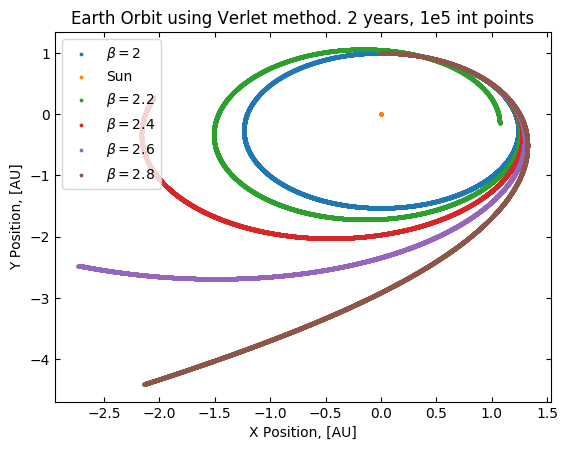
\includegraphics[width=0.8\textwidth]{Earth-Sun_beta.png}
  \caption{Escape velocity with increasing exponent of denominator of the gravitational force.}
  \label{fig:v_esc_beta}
\end{figure}
\FloatBarrier
All this was found using the initializer found in \href{https://github.com/kmaasrud/Project-5/blob/master/code/complete_solar-system/src/initialize_test.cpp}{\textsc{/src/initializer\_test.cpp}} inside our \textsc{complete\_solar-system} code folder by changeing the initial velocity of the Earth, and changing the exponent of the distance $r$ on line $40$ in our body-code found in \href{https://github.com/kmaasrud/Project-5/blob/master/code/complete_solar-system/src/body.cpp}{\textsc{/src/body.cpp}}. Then the plotter found in \href{https://github.com/kmaasrud/Project-5/blob/master/code/Plotter/2d-plot_beta.py}{\textsc{/Plotter/2d-plot\_beta.py}} was used to plot the figure above.

%oppgave 5e)
\subsection{Three-body problem: Sun, Earth and Jupiter.}
The first four plots below show the three-body simulation when the sun is fixed, with varying masses of Jupiter.

\begin{figure}[!h]
  \centering
  \makebox[\textwidth][c]{
  \begin{minipage}{0.7\textwidth}
        \centering
        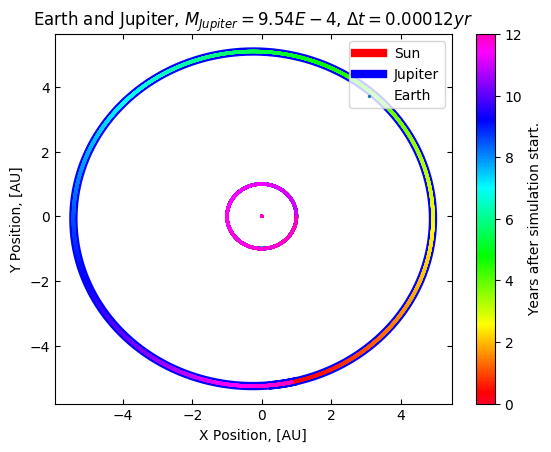
\includegraphics[width=1\textwidth]{jupiter-1_fixed.png} % first figure itself
    \end{minipage}\hfill
    \begin{minipage}{0.7\textwidth}
        \centering
        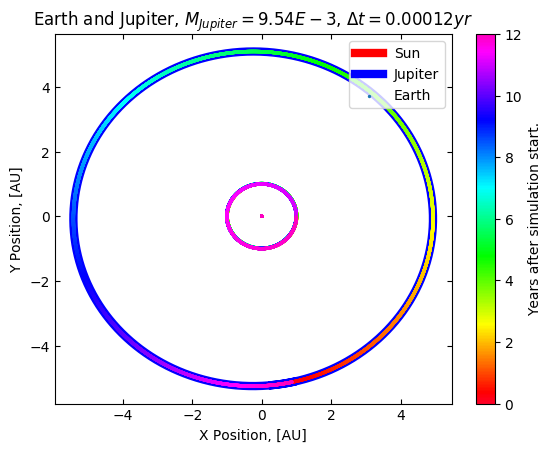
\includegraphics[width=1\textwidth]{jupiter-10_fixed.png} % second figure itself
    \end{minipage}}
  \caption{Positions of Sun in the middle, Earth second and outermost Jupiter calculated using the velocity Verlet method with with original mass of Jupiter and an increase of mass of a factor of 10 respectively. The sun is in a fixed position.}
  \label{fig:SunEarthJupiter10fixed}
\end{figure}

\begin{figure}[!h]
  \centering
  \makebox[\textwidth][c]{
  \begin{minipage}{0.7\textwidth}
        \centering
        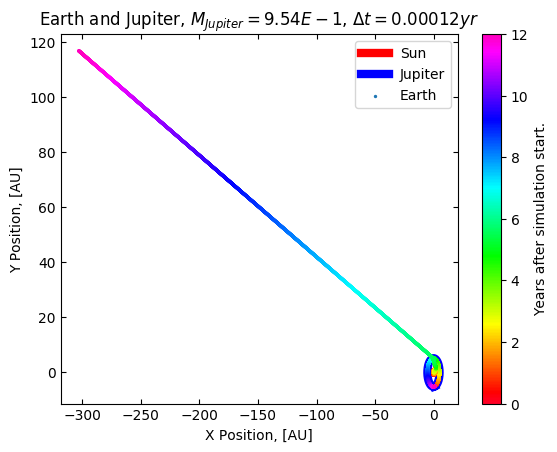
\includegraphics[width=1\textwidth]{jupiter-1000_fixed.png} % first figure itself
    \end{minipage}\hfill
    \begin{minipage}{0.7\textwidth}
        \centering
        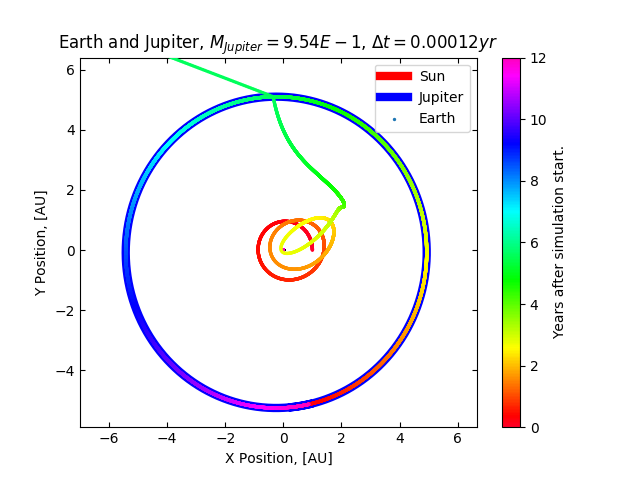
\includegraphics[width=1\textwidth]{jupiter-1000_Closeup_fixed.png} % second figure itself
    \end{minipage}}
  \caption{Positions of Earth and Jupiter using the velocity Verlet method with an increase of mass with a factor of 1000. After approximately 5 years, Earth escapes the system. The illustration to the right is a magnified version of the first plot and shows the three body interaction when the sun is fixed.}
  \label{fig:SunEarthJupiter10000fixed}
\end{figure}
\FloatBarrier

In order to test the fixed sun approximation, we also calculated this scenario for a dynamic Sun, shown below.

\begin{figure}[!h]
  \centering
  \makebox[\textwidth][c]{
  \begin{minipage}{0.7\textwidth}
        \centering
        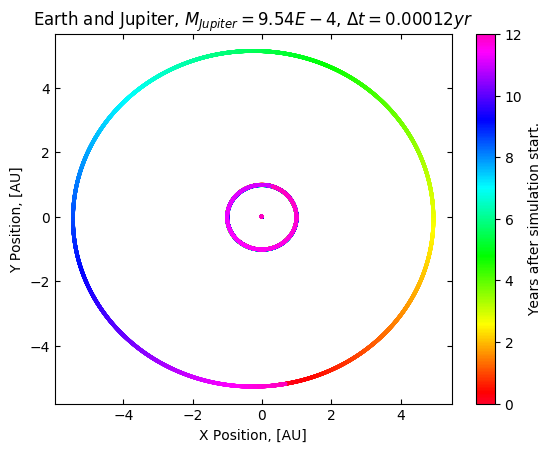
\includegraphics[width=1\textwidth]{jupiter-1.png} % first figure itself
    \end{minipage}\hfill
    \begin{minipage}{0.7\textwidth}
        \centering
        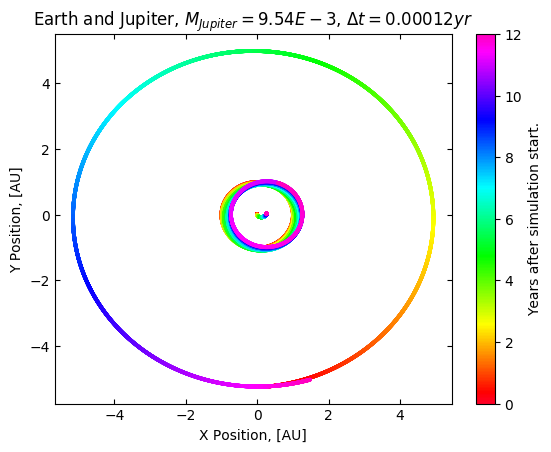
\includegraphics[width=1\textwidth]{jupiter-10.png} % second figure itself
    \end{minipage}}
  \caption{Positions of Sun in the middle, Earth second and outermost Jupiter calculated using the velocity Verlet method with with original mass of Jupiter and an increase of mass of a factor of 10 respectively}
  \label{fig:SunEarthJupiter10}
\end{figure}

\begin{figure}[!h]
  \centering
  \makebox[\textwidth][c]{
  \begin{minipage}{0.7\textwidth}
        \centering
        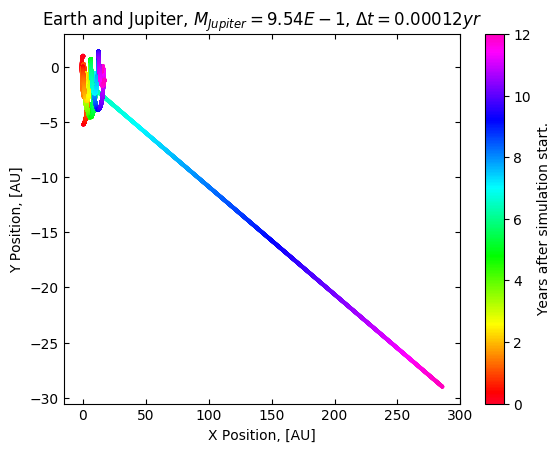
\includegraphics[width=1\textwidth]{jupiter-1000.png} % first figure itself
    \end{minipage}\hfill
    \begin{minipage}{0.7\textwidth}
        \centering
        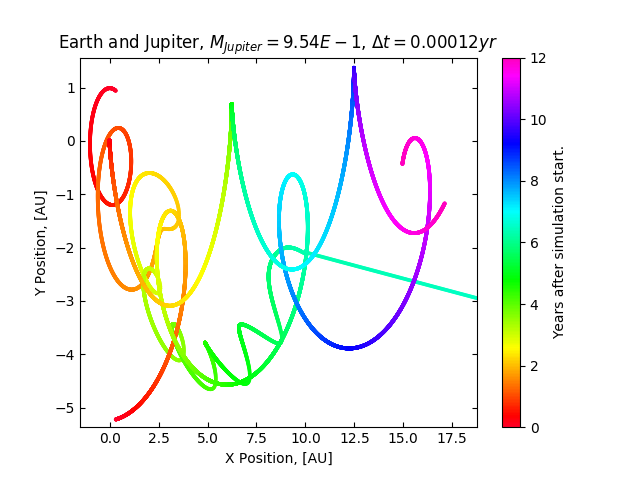
\includegraphics[width=1\textwidth]{jupiter-1000_Closeup.png} % second figure itself
    \end{minipage}}
  \caption{Positions of Earth and Jupiter using the velocity Verlet method with an increase of mass with a factor of 1000. After approximately 7 years, Earth escapes the system. The illustration to the right is a magnified version of the first plot and shows the beautiful interaction between two equally heavy objects.}
  \label{fig:SunEarthJupiter10000}
\end{figure}
\FloatBarrier
Stability Verlet solver with increased mass:


%oppgave 5f)
\subsection{The Solar system} \label{sec:results-entire-solar-system}
Finally we will add all the other planets to make the Solar system complete, still using the Verlet solver. Rather than having the origin in the postion of the sun, we are using the Barycenter of our solar system. All initial conditions were taken from NASA's HORIZONS web interface\cite{HorizonsNASA} with a date of December 4.

\begin{figure}[!h]
\centering
  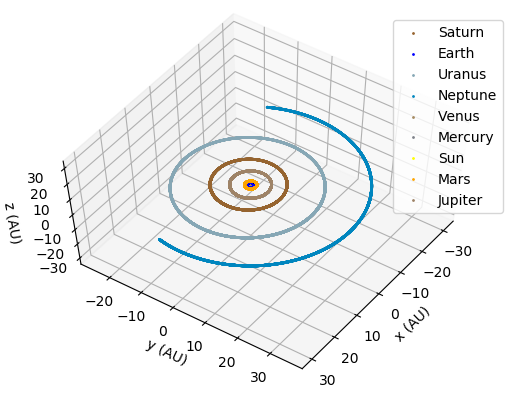
\includegraphics[width=0.7\textwidth]{allPlanets.png}
  \caption{All planets in The Solar System. Due to the large orbits of the outer planets, it is hard to plot the orbit of the inner planets, the Sun, Venus and Mercury without loosing information from the outermost planets.}
  \label{fig:allPlanets}
\end{figure}


\subsection{The perihelion precession of Mercury}
By using initial conditions of $2 \cdot 10^8$ integration points over a century, we are using a timestep $\Delta t = 5\cdot 10^{-7}$, which is really small. We also changed the code to only save the position of Mercury to file in the last year of simulation to save space. The initializer used is found in \href{https://github.com/kmaasrud/Project-5/blob/master/code/complete_solar-system/src/initialize_perihelion.cpp}{\textsc{/src/initializer\_perihelion.cpp}} inside our \textsc{complete\_solar-system} code folder.

\begin{table}[!h]
  \centering
  \caption{Table of Mercury's calculated perihelion precession with and without relativistic correction.}
  \begin{tabular}{c c}
    & $\theta_p$(Degrees)\\
    \hline
    Newtonian &  $-0.000426^\circ$\\
    Relativistic &  $0.0117318^\circ$\\
  \end{tabular}
\end{table}
\FloatBarrier

\end{document}
